
\documentclass[12pt,pdftex, notitlepage]{article}
%%%%%%%%%%%%%%%%%%%%%%%%%%%%%%%%%%%%%%%%%%%%%%%%%%%%%%%%%%%%%%%%%%%%%%%%%%%%%%%%%%%%%%%%%%%%%%%%%%%%%%%%%%%%%%%%%%%%%%%%%%%%
\usepackage[pdftex]{graphicx}
\usepackage[nomessages]{fp}
\usepackage[usenames,dvipsnames]{color}
\usepackage{amsmath, amsthm, amssymb}
\usepackage[hyphens]{url}
\usepackage{fullpage}
\usepackage{bbm}
\usepackage{setspace}
\usepackage{float}
\usepackage{verbatim}
\usepackage{pdfpages}
\usepackage{lscape}
\usepackage{booktabs}
\usepackage{multirow}
\usepackage[english]{babel}
%\usepackage{tabulary}
\usepackage{tabularx}
\usepackage{array}
\usepackage{sectsty}
\usepackage{pdflscape}
\sectionfont{\large}
\usepackage{xfrac}
 \usepackage[normalem]{ulem}
\newcommand{\sups}[1]{\ensuremath{^{\textrm{#1}}}}
\newcommand{\subs}[1]{\ensuremath{_{\textrm{#1}}}}
\usepackage{pgfplots}
\usepackage{soul}
\usepackage{caption}
\usepackage{subcaption}
\usepackage{tabularx}

\usepackage{clipboard}
\newclipboard{example}

\usepackage{xr} 

%Here I add some functionality to the bibliography, to allow it to have separate lists of references for different parts of the document (main paper, and then each appendix section) ;
\usepackage[backend=biber, natbib=true, style=authoryear, giveninits=true, doi=false,isbn=false,url=false]{biblatex}

\DefineBibliographyStrings{english}{%
  references = {\large References},
}

%%Calling the bib file
\bibliography{fakebib2} 

%Just allows creation of graphics
\usepackage{tikz}
\usepackage{graphicx}
\usetikzlibrary{arrows}
\usetikzlibrary{decorations.markings}
\usetikzlibrary{decorations.pathreplacing}


\floatstyle{plain}

\let\footnotesize=\small
\let\titlesize=\small

\usepackage{geometry}
\geometry{verbose,letterpaper,tmargin=1.0in,bmargin=1in,lmargin=1in,rmargin=1in}


\singlespacing

\begin{document}

%%%This line below begins one section of the references (in this case, for the main part of the paper)
\begin{refsection}

\author{Bodie Katz and Ilyana Kuziemko}
\title{\vspace{-2.5cm}\Large{Fake Paper to Document Some Useful Tricks in \LaTeX }\thanks{We thank our brilliant editor and two insightful, anonymous referees.}}
\date{\today}

\maketitle
\begin{abstract}
\noindent
This is just some fake content (gibberish) to demonstrate tricks for revising a paper in response to referee and editor comments.  
\end{abstract}


\thispagestyle{empty}

\newpage

\onehalfspacing
\setcounter{page}{1}

\section{Introduction}\label{sec-intro}

%This paragraph below I want to copy into the referee response letter. so I set it off with this \Copy{intro_par} and then call it in the response memo by typing "\Paste{into_par}"
%We also want to grab the page number for the referee letter (so i label intro-page and then in the response memo can tell the referee which page to look at by typing "\pageref{intro-page}".
\label{intro-page} \Copy{intro_par}{In this paper we make three make contributions.  First, we extend the sample period used in the seminal work of \citet{piketty2003income}.  Second, we apply re-weighting methods as in \citet{dinardo1996labor}.  Third, we develop an instrumental-variable strategy based on plausibly exogenous variation in differences between the lunar and Gregorian calendars.}

\section{Model}\label{sec-model}

A complete model is presented in Appendix \ref{app-sec-model}.  Here, we sketch the basic intuition.

Assume a four-period model with two boundedly rational agents and a social planner with Rawlsian preferences and a discount rate of zero.  Our model borrows liberally from \citet{mirrlees1971} and \citet{harry_potter}.

\section{Empirical strategy}\label{sec-strategy}

The underlying logic of empirical strategy is that holidays provide workers free time away from the labor market, allowing them time to organize.  In some years, the lunar and Gregorian calendars correspond to provide a greater number of holidays, providing quasi-random variation in the number of holidays and thus time for working to organize into unions.  We thus hypothesize that there is a strong, positive relationship between union density and the number of holidays in a give year $t$.

Our empirical strategy is clearly illustrated in Figure \ref{fig-first-stage}.

\section{Results}\label{sec-results}

Table \ref{tab-main} depicts the main results.  The first stage shows a strong relationship between years where there are a confluence of lunar- and Gregorian-calendar holidays and greater union density.  Contrary to our hypothesis in Section \ref{sec-strategy}, the coefficient on the \textit{Holidays} variable is negative, so we now hypothesize that a greater number of holidays reduces the ability of workers to organize into unions (due, naturally, to greater distraction).

The second-stage results support the main hypothesis that union density reduces inequality.  Greater union density increase the labor-share of income and reduces the top-ten-share of income.

\section{Robustness}\label{sec-robust}

A natural question is which holidays to include in the instrumental variable.  In Appendix Table \ref{tab-main-robust} we add to the regression in Table \ref{tab-main} a control for minor holidays, including those from the Chinese calendar.\footnote{The minor holidays we add include Arbor Day, Flag Day, and Groundhogs Day. \label{minor-holidays}}  Remarkably, the results are unchanged.

\section{Conclusions}

Our work raises many questions that we believe will be fruitful ground for future research.  


\singlespacing

\printbibliography
\end{refsection}


\newpage \clearpage 


\begin{figure}[p]
	\caption{Illustration of first-stage variation} \label{fig-first-stage}
	\centerline{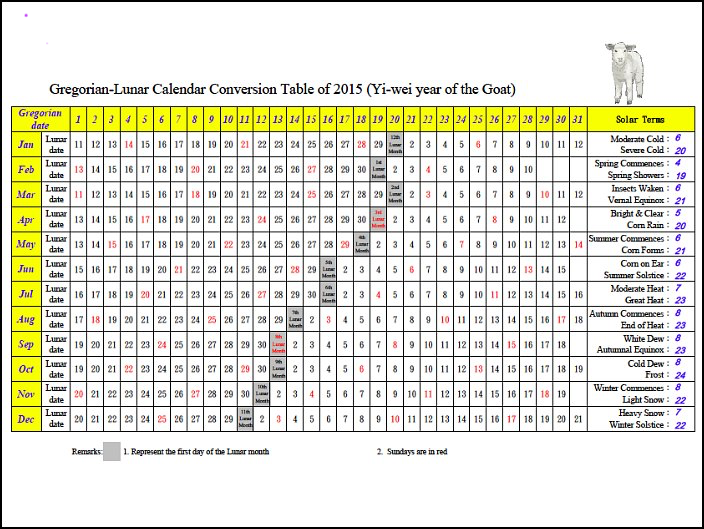
\includegraphics[width=7in]{figures/lunar-calendar.png}}
	\raggedright
	\footnotesize{\textit{Data sources}: XXXX. \\
\vspace{.3cm}	
\noindent \raggedright	\textit{Notes}:  XXX.}

\end{figure}



\begin{table}
\setlength{\tabcolsep}{1pt}
\def\sym#1{\ifmmode^{#1}\else\(^{#1}\)\fi}
\caption{Aggregate inequality as a function of union density \label{tab-main}}
\scriptsize{
\begin{tabular*}{1.0\hsize}{@{\hskip\tabcolsep\extracolsep\fill}l  cc cc cc cc   }
\toprule
\input tables/fake_first_stage.tex
\bottomrule
\end{tabular*}
}
\raggedright
\footnotesize{\textit{Sources}: XXX.

\vspace{.3cm}

\textit{Notes:} XXX.
}
\end{table}

\newpage \clearpage
\appendix
\makeatletter
\def\@seccntformat#1{\csname named#1\endcsname\csname the#1\endcsname.\quad}
\makeatother
\newcommand{\namedsection}{Appendix }

%%%%%%%%%%%%%%%%%%%%%%%%%%%%%%%%%%%%%%%%%%%%%%%%%%%%%%%%
%%%%%%%%%%%%%%%%%%%%%%%%%%%%%%%%%%%%%%%%%%%%%%%%%%%%%%%%
%%%%%%%%%%%%%%%%%%%%%%%%%%%%%%%%%%%%%%%%%%%%%%%%%%%%%%%%
%%%%%%%%%%%%%%%%%%%%%%%%%%%%%%%%%%%%%%%

%%%%%%% APPENDIX FIGURES  AND TABLES
\section{Supplementary results noted in the text  \label{app_figs_tables}}
%%%%%%%%%%%%%%%%%%%%%%%%%%%%%%%%%%%%%%%

\setcounter{figure}{0}
\renewcommand{\figurename}{Appendix Figure}
\setcounter{table}{0}
\renewcommand{\tablename}{Appendix Table}

\renewcommand{\thetable}{\thesection.\arabic{table}}
\renewcommand{\thefigure}{\thesection.\arabic{figure}}


\begin{table}[h]
%\setlength{\tabcolsep}{1pt}
\def\sym#1{\ifmmode^{#1}\else\(^{#1}\)\fi}
\caption{Main results, robustness to including minor holidays \label{tab-main-robust}}
\scriptsize{
\begin{tabular}{l  cc cc cc cc   }
\toprule
\input tables/fake_first_stage_minor.tex
\bottomrule
\end{tabular}
}
\raggedright
\footnotesize{\textit{Notes:} The specifications are identical to those in Table \ref{tab-main} except that here we add controls for minor holidays.}
\end{table}


\newpage \clearpage
%%%%%%%%%%%%%%%%%%%%%%%%%%%%%%%%%%%%%%%
\section{Formalization of the model}\label{app-sec-model}
%%%%%%%%%%%%%%%%%%%%%%%%%%%%%%%%%%%%%%%

\setcounter{figure}{0}
\renewcommand{\figurename}{Appendix Figure}
\setcounter{table}{0}
\renewcommand{\tablename}{Appendix Table}

\renewcommand{\thetable}{\thesection.\arabic{table}}
\renewcommand{\thefigure}{\thesection.\arabic{figure}}

Our model is clearly illustrated in Appendix Figure \ref{fig-model}.


\vspace{2cm}

\begin{figure}[h]
	\caption{Illustration of the theory} \label{fig-model}
	\centerline{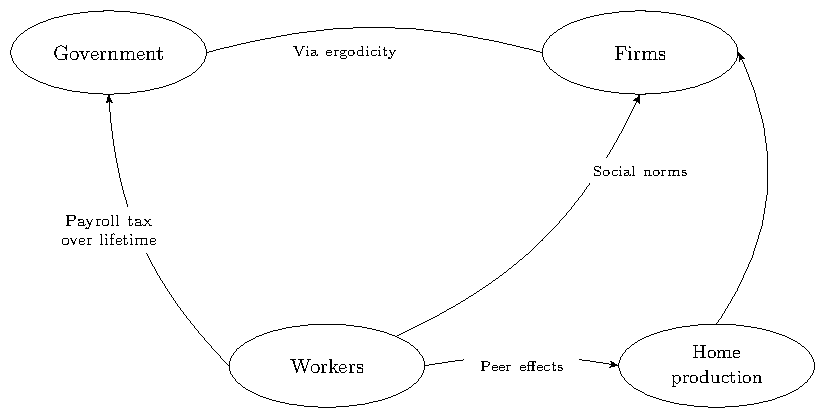
\includegraphics[width=7in]{figures/fake_model_flow.pdf}}
	
\noindent \raggedright	
\footnotesize{\textit{Notes}:  XXX.}

\end{figure}

\newpage \clearpage

%%%%%%%%%%%%%%%%%%%%%%%%%%%%%%%%%%%%%%%


\section{History of the lunar and Gregorian calendars}\label{app-sec-calendar}



%%%%%%%%%%%%%%%%%%%%%%%%%%%%%%%%%%%%%%%

\setcounter{figure}{0}
\renewcommand{\figurename}{Appendix Figure}
\setcounter{table}{0}
\renewcommand{\tablename}{Appendix Table}

\renewcommand{\thetable}{\thesection.\arabic{table}}
\renewcommand{\thefigure}{\thesection.\arabic{figure}}

We digitize calendars from the Ancient, Julian and Gregorian periods.  See Appendix Figure \ref{fig-old-calendar} for an example of the material we digitize.

For further background, please see  \citet{depuydt1997civil} and \citet{mckay2016coligny}.


\begin{figure}[h]
	\caption{Example of ancient calendar} \label{fig-old-calendar}
	\centerline{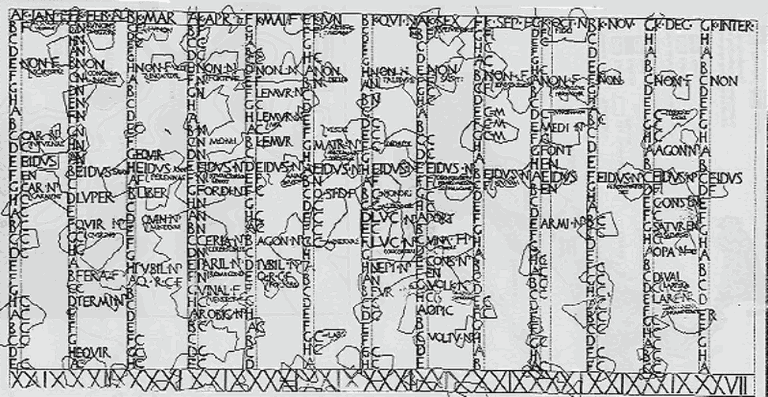
\includegraphics[width=7in]{figures/old_calendar.png}}
	
\noindent \raggedright	
\footnotesize{\textit{Notes}:  XXX.}
\end{figure}





\end{document}



